\documentclass{amsart}
\usepackage{graphicx}
\graphicspath{{./}}
\usepackage{hyperref}
\usepackage{csvsimple}
\usepackage{longtable}
\usepackage{epigraph}
\title{Stronger Evidence For Hobbes Exponential Tails}
\author{Zulfikar Moinuddin Ahmed}
\date{\today}
\begin{document}
\maketitle

\section{Recap of Hobbes Exponential Tails for Moral Values}

I have in the recent weeks been concerned with understanding deviations from what I call Rousseau Exponential Distributions for Human Moral Values.  An examination of the measured distribution of Justifiability of political violence led to my invention of the Log-V distribution.

These look like this.

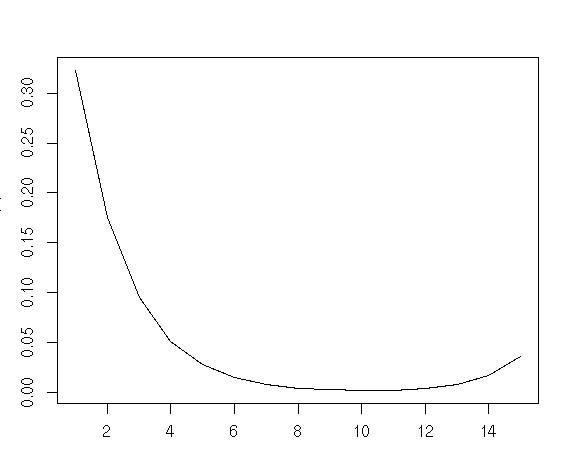
\includegraphics[scale=0.8]{synthterror.jpeg}

I won't go into technical details on fitting these here.

In this note I would like to present some evidence that this model is appropriate for actual data from Nature.  This is the substantial point.  We are always aware that our scientific models are {\em artificial inventions} and that Nature has no obligation to behave by them.  And yet once in a while, great fortune and serendipity leads to models that will adequately describe natural data.

My idea of the Hobbes Exponential Tail was a speculative hypothesis, relatively recent, early May 2021.  And my heart is filled with joy and gratitude to see that Nature has found some agreement with the idea, always the great hope of any man who has invested many years in the pursuit of Science.  

I made the discovery today that for extreme agreement that political violence is justified, (levels 9 and 10 out of 1--10), the conditional distribution of a range of moral questions Q177--Q195 all have abnormal tail distributions.  

This gives us quite a few examples of Natural data where we can check our hypothesis.

We consider the following exercise.  All of the conditional distributions are 10-vectors.  We consider the 'time-reversed' vector $v$ and consider whether $v[1:4]$ has exponential fit.  

\section{Q177--Q195 time-reversed exponentials}

% latex table generated in R 4.0.3 by xtable 1.8-4 package
% Tue May  4 02:07:07 2021
\begin{table}[ht]
\centering
\begin{tabular}{rlrr}
  \hline
 & var & lambda & rsq \\ 
  \hline
1 & Q177 & -0.6586 & 0.7442 \\ 
  2 & Q178 & -0.7192 & 0.8613 \\ 
  3 & Q179 & -0.8945 & 0.8884 \\ 
  4 & Q180 & -0.7321 & 0.7967 \\ 
  5 & Q181 & -0.7457 & 0.8072 \\ 
  6 & Q182 & -0.7101 & 0.8513 \\ 
  7 & Q183 & -0.7709 & 0.8384 \\ 
  8 & Q184 & -0.6475 & 0.7056 \\ 
  9 & Q185 & -0.6112 & 0.7328 \\ 
  10 & Q186 & -0.6470 & 0.8068 \\ 
  11 & Q187 & -0.7904 & 0.7402 \\ 
  12 & Q188 & -0.6540 & 0.7536 \\ 
  13 & Q189 & -0.9370 & 0.8857 \\ 
  14 & Q190 & -0.7191 & 0.8510 \\ 
  15 & Q191 & -0.9505 & 0.9345 \\ 
  16 & Q192 & -0.2442 & 0.2000 \\ 
  17 & Q193 & -0.6229 & 0.7606 \\ 
  18 & Q194 & -0.8782 & 0.8706 \\ 
  19 & Q195 & -0.7860 & 0.8265 \\ 
   \hline
\end{tabular}
\end{table}

The miss Q192 is the terrorism agreement variable, and can be ignored.    Excluding this variable, mean $R^2=0.814$ with standard deviation 0.06.  This is extremely strong vindication of Hobbes Tail Exponential as a feature of Nature.  

I am most gratified, for the Rousseau Exponential was discovered by myself for moral variables, and it was quite a difficult examination that led to the reversed exponential distribution at their tails and we can now be fairly confident that these are not arbitrary artifacts but actual features of human nature.

\section{Are these Evil People At the Tail?}

We have to be careful to consider people Evil; very rarely -- such as in the case of Bill Gates -- we do have fundamentally Evil Demon Soul in a human body.  These are people who have lost their way in moral development, and I speculate that their moral character failed during adolescence, and so they embraced extreme criminal views.  These span all ethnicities, and they are about 2.5\% of white people in the world.  For other ethnicities they vary a bit but lower than around 2.5\% generally.  These are people whose moral values are Hobbesian more than Rousseau-ean which will be roughly 95\% of people of all ethnicities.  
\end{document}